% \documentclass[jou,apacite]{apa6}
\documentclass[doc,apacite,12pt]{apa6}

%-------------------------
 % Packages

\usepackage[normalem]{ulem}
\usepackage{listings}

\usepackage{url}

\usepackage{graphicx}
\graphicspath{ {resources/} }

\usepackage{minted}

\usepackage{wrapfig}

%-------------------------
 % Commands
\newcommand{\bx}{BlaTeX }
\newcommand{\lx}{LaTeX } 
%Need space after to make sure the space is inserted after command

%-------------------------
 % The Title of your paper

\title{BlaTeX}
\shorttitle{R. Shah}

%-------------------------
 % Author

\author{Rushi Shah}
\affiliation{TJHSST}

%-------------------------
 % Abstract               
%-------------------------
\abstract{BlaTeX is a static-site compiler for LaTeX posts written in Haskell. It is a Haskell program that a user can invoke through a command-line interface; it consumes a directory full of LaTeX source code files and their output and generates a static HTML/PDF website for those posts. The project is mainly focused on users who would like to maintain a blog about their academic/professional/personal work in computer science or mathematics. }

\begin{document}
\maketitle    


% TODO:
% Abstract
% Results, Discussion, and Conclusion
% Citations
         
%-------------------------
 % Introduction               
%-------------------------
\section{Introduction}
%Motivation for research.

Markdown and HTML are the standard tools used to write standard tech blogs with. But they have weak support for embedding mathematical formulas, and are not conducive to writing for an extended period of time. So instead of writing posts in Markdown, my project allows writers to create posts in LaTeX (a powerful type-setting and markup language) and generate a static-site that can be deployed to any hosting service.

%-------------------------
 % Background 
%-------------------------
\section{Background}

My project, called BlaTeX, is a static-site compiler written in Haskell that compiles LaTeX posts into a deploy-able site. It is inspired by a similar Ruby tool called Jekyll that compiles Markdown posts into a static, deploy-able site. However, it allows the user to write posts in LaTeX rather than Markdown (because LaTeX is a more powerful tool) and is overall a more lightweight blogging software. 

% Typically, static-sites like blogs are built with a tool called Jekyll. This Ruby project compiles Markdown posts into a static HTML site. \bx is similar, it is a static-site compiler written in Haskell that compiles LaTeX posts into a deploy-able site. The following description has been edited to highlight the minor differences between Jekyll and \bx:

% \sout{Jekyll} BlaTeX is a simple, blog-aware, static site generator. It takes a template directory containing \sout{raw text files in various formats} LaTeX files\sout{, runs it through a converter (like Markdown) and our Liquid renderer,} and spits out a complete, ready-to-publish static website suitable for serving with your favorite web server. \sout{Jekyll also happens to be the engine behind GitHub Pages, which means} you can use \sout{Jekyll} BlaTeX to host your project's page, blog, or website from GitHub's servers for free.

Another popular content-management system for blogging is Wordpress. However, Wordpress posts are edited in the Wordpress Administration Panel as ``What you see is what you get''. Neither Markdown nor LaTeX are ``What you see is what you get'', and thus Wordpress caters to a different audience (a group of mostly non-technical authors). 

%-------------------------
 % Development
%-------------------------
\section{Development \& Techniques}

\subsubsection{Requirements}
  % Technical requirements should be more about the requirements that would make this project a success
  This command line utility requires the Haskell Platform and LaTeX. The Haskell Platform includes GHC (a Haskell compiler) and Cabal, which is Haskell's primary package manager. LaTeX is needed to build LaTeX posts into their resulting PDFs. After the Haskell Platform has been installed, installing BlaTeX is simple:

  \begin{lstlisting}
  > cabal install blatex
  \end{lstlisting}

\subsubsection{Overview}
  % Briefly outline the method used to develop the project
  The project is a command line utility that is written in Haskell. Haskell is a statically-typed functional programming language that makes heavy use of the REPL. Libraries were tested/experimented with independently in their own files. After the necessary functions were written, they were integrated into the final product. The finished project was assembled into an executable file and deployed to Haskell's package manager (Hackage). 

\subsubsection{Limitations}
  % Equipment, time, materials, etc.

  One potential limitation of this project is that it only compiles links to PDF files. Because LaTeX can't generate HTML, the blog will only be a series of interlinked PDF files rather than a series of interlinked HTML files. This is not necessarily a limitation, but it may interrupt the status quo of typical blogs made of HTML pages. 

  % In order to parse the user's LaTeX files into an abstract syntax tree that can be consumed by Haskell, this project uses a Haskell package called \texttt{HaTeX}. This is a wonderful package (most of the time). The problem arises in a specific parsing instance. In LaTeX, a math environment is defined between two dollar-signs (\texttt{\$MATH GOES HERE\$}). In order to use dollar-signs as actual dollar-signs (like ``You owe me \$5''), you use an escape character before the symbol (\textbackslash). This is an exception to the math environment rule. However, HaTeX is not programmed to catch this exception gracefully. It matches pairs of dollar-signs and treats everything in between as math. If there are an odd number of dollar signs, or only one (even if they are escaped properly) HaTeX will just flat out fail to parse the entire file and thus BlaTeX will similarly ignore the post. 

  Dates are formatted in \texttt{DD MONTH YEAR} which contributes to the minimalist, classy theme of PDF blog posts; this date format is also used in the internal implementation. However, this becomes an issue if multiple posts are authored on same day because they will not be displayed in the correct order. 

\subsection{Research Theory and Design Criteria}
  % Clearly and Thoroughly present project methods, theory and algorithms
  % Expand upon process in detail – (what you did), making sure to represent a sufficient level of difficulty and complexity
  \subsubsection{Error Handling}
    Error handling was one of the most complex aspects of this project. Haskell is a strongly typed language and utilizes Type Classes for a large portion of functionality to produce elegant and expressive code. Series of functions that could potentially create errors were chained together with an instance of an Applicative Functor. Originally the Maybe Applicative was used, but in order to produce meaningful error messages for the user, I switched to the Either Applicative. A simplified example of code used to handle some potential errors is as follows:
    
    \begin{minted}{haskell}
createPost s t = Post <$> pure s <*> title <*> author <*> date <*> pure t
  where 
    date = (getCommandValue "date" t)
    author = (getCommandValue "author" t)
    title = (getCommandValue "title" t)
    \end{minted} 

    In this code, the \texttt{getCommand} function will either find the command within the abstract syntax tree, or the given command was never used. If the command was never used, no post can be created because the requisite information was missing. This series of function calls are tied together with \texttt{<*>}, the ``splat'' operator on Applicative instances. If one computation fails, the ultimate computation will also fail.  

  \subsubsection{Input/Output}
    Because Haskell is a purely functional programming language, no side effects are permitted. This makes input/output rather difficult, and thus \texttt{Monad}'s are used to simulate the desired side effects. However, ubiquitous use of Monads defeats the purpose of the purely functional nature of Haskell. Thus, the input-output code was confined to a single module where almost all effect-ful computations were handled. The main function was included here that glued together all pure functions. This function included code to automatically initate the proper file structure and skeleton files for a new user through system commands. It also included code for the building process. The output of this process is:

    \begin{verbatim}
Getting directory contents
Turning directory contents into posts
All posts are well formed
Turning posts into an HTML element
Reading the layout file
Inserting HTML element into layout file
Writing resulting file into index.html
Success building!
    \end{verbatim} 

    If an error is raised at any point in the process, the process will halt and display the error message for the user to troubleshoot. 

\subsection{Developmental Procedures}
  % Explain the steps you took such that your project could be repeated by others (how you did it)

  In general terms: a directory containing posts is examined by BlaTeX, each post is parsed into an abstract syntax tree, information from this tree is parsed into a Haskell Post data structure, each post is stored into a list, the list is sorted by the date, each object is converted into it's corresponding HTML, and this HTML is outputted into an output file at a user-specified location. 

  \subsubsection{The \texttt{Post} Algebraic Data Strucure}

    In Haskell, the equivalent of an ``object'' (used in object oriented programming languages), is an ``algebraic data type (ADT)''. To represent each post, a \texttt{Post} algebraic data type was defined with meta-information for each post. The final definition for the Post was:

    \begin{minted}{haskell}
data Post = Post {
  fileName :: String
  , postTitle :: String
  , postAuthor :: String
  , postDate :: DateTime
  , syntaxTree :: LaTeX
    }
    deriving (Eq, Show)
    \end{minted}

  This defines the structure of a Post based on each attribute it would have and what type that attribute would have.

  \subsubsection{BlazeHTML}
    The first part of the project that I tacked was generating HTML elements that would need to be inserted into the final file. Each post object would generate the following LI element:

  \begin{minted}{html}
<li class='blog-post'>
    <a class='post-link' href='posts/example-post.pdf'>
        Example Post
    </a>
    <div class='post-date'>
        1 January 2015
    </div>
</li>
  \end{minted}

  \subsubsection{HaTeX}
    The second part of the project required that I read in LaTeX files for the posts and use them to extract certain meta-information about each post. This included the title of the post (inserted into the \texttt{.post-link} tag) and the date of the post (used to sort posts and displayed in the \texttt{.post-date} tag). 

  \subsubsection{TagSoup}

    The user supplies a layout file which defines the format and style of their blog. BlaTeX finds the line \texttt{<ul id='blog-posts'></ul>} and inserts all the posts at that point. In order to do so, the project reads in an HTML file and derives it's abstract syntax tree with a package called TagSoup. TagSoup converts an HTML file into a list of HTML elements, and the HTML generated with BlazeHTML is inserted at the specified point. 

  \subsubsection{Dates}

    Support for dates was one of the final undertakings addressed. The Data.Dates package was used to parse the LaTeX dates. This allowed me to sort the list of posts chronologically.  

\subsection{Internal Testing and Analysis}
  % How did you test and validate your code?
  Because this tool was written in Haskell (a statically-typed, compiled programming language), most insidious bugs were filtered out at compile time. Haskell development is also strongly integrated with using a Haskell REPL (read-eval-print-loop). Thus, each function was experimented with in the REPL after being written and before being pushed to production. 


\clearpage

\subsection{User Interface Testing and Analysis}
  % Explain your user validation test
  % Present the results of your user validation test
  % I literally used it to maintain my own blog

  \begin{wrapfigure}{r}{0.6\textwidth}
    % \begin{center}
      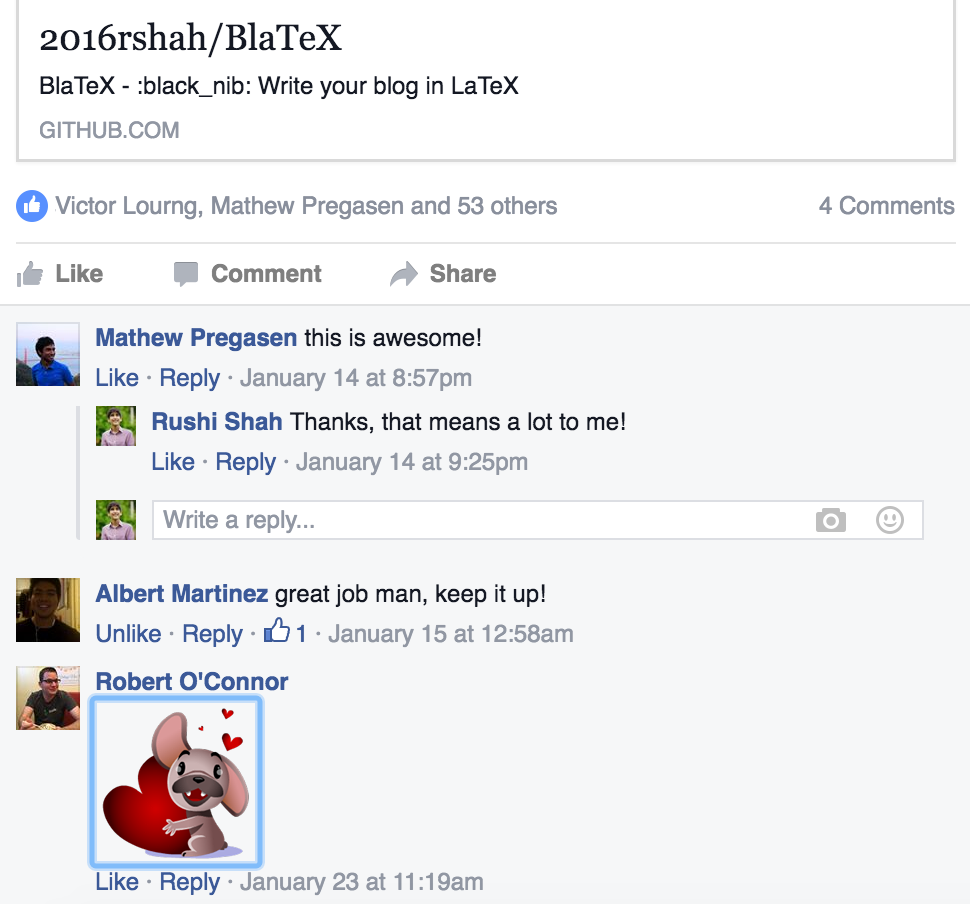
\includegraphics[width=0.6\textwidth]{facebook}
    % \end{center}
    \centering
  \end{wrapfigure}

  In order to test this project, I used it to create and maintain \url{http://rshah.org/blog}. Through my own use I discovered multiple improvements that could be made to the user interface and experience, which I promptly implemented. 

  I also posted my project in a Facebook group for functional programming and recieved an overwhelmingly positive response: 

  % \centerline{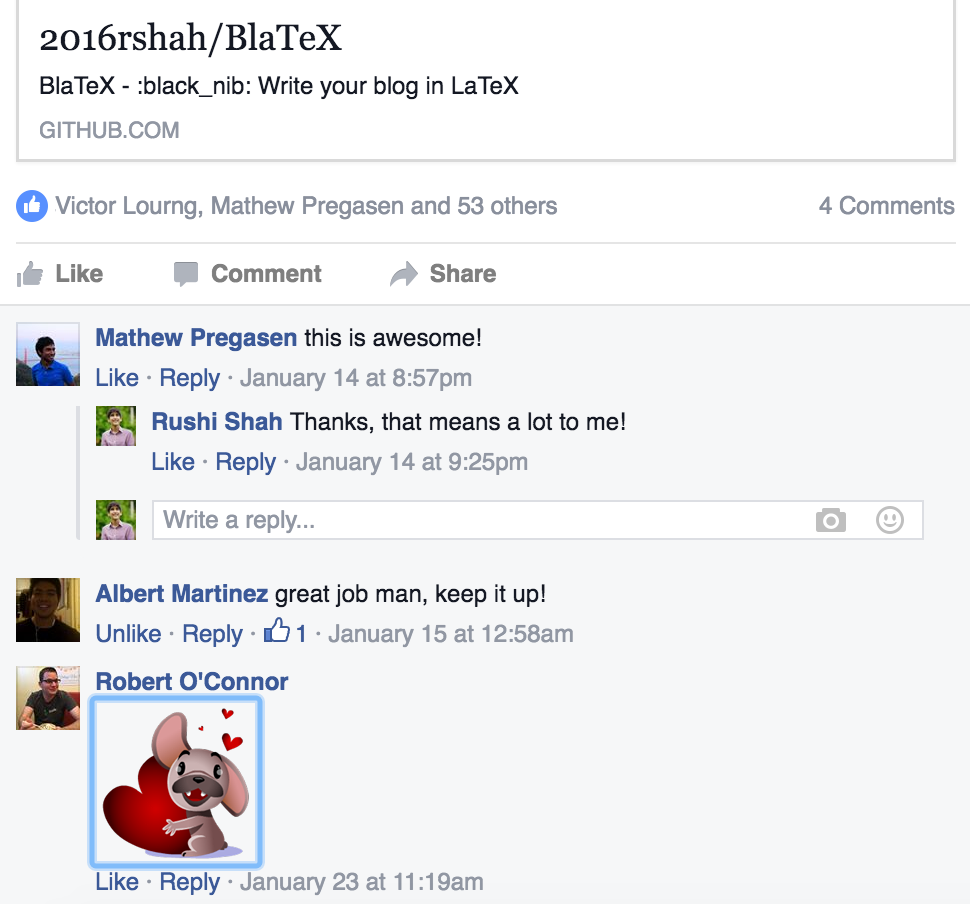
\includegraphics[width=.8\textwidth]{facebook}}

  It is also an open source project on Github, and met a similarly positive reaction from that community (with 19 Github ``stars''). 

\subsection{Visual representation of Results}
  % Visually represent your project’s structure, results, algorithms

  My blog at \url{http://rshah.org/blog} is a visual representation of a static site compiled with BlaTeX.

  \centerline{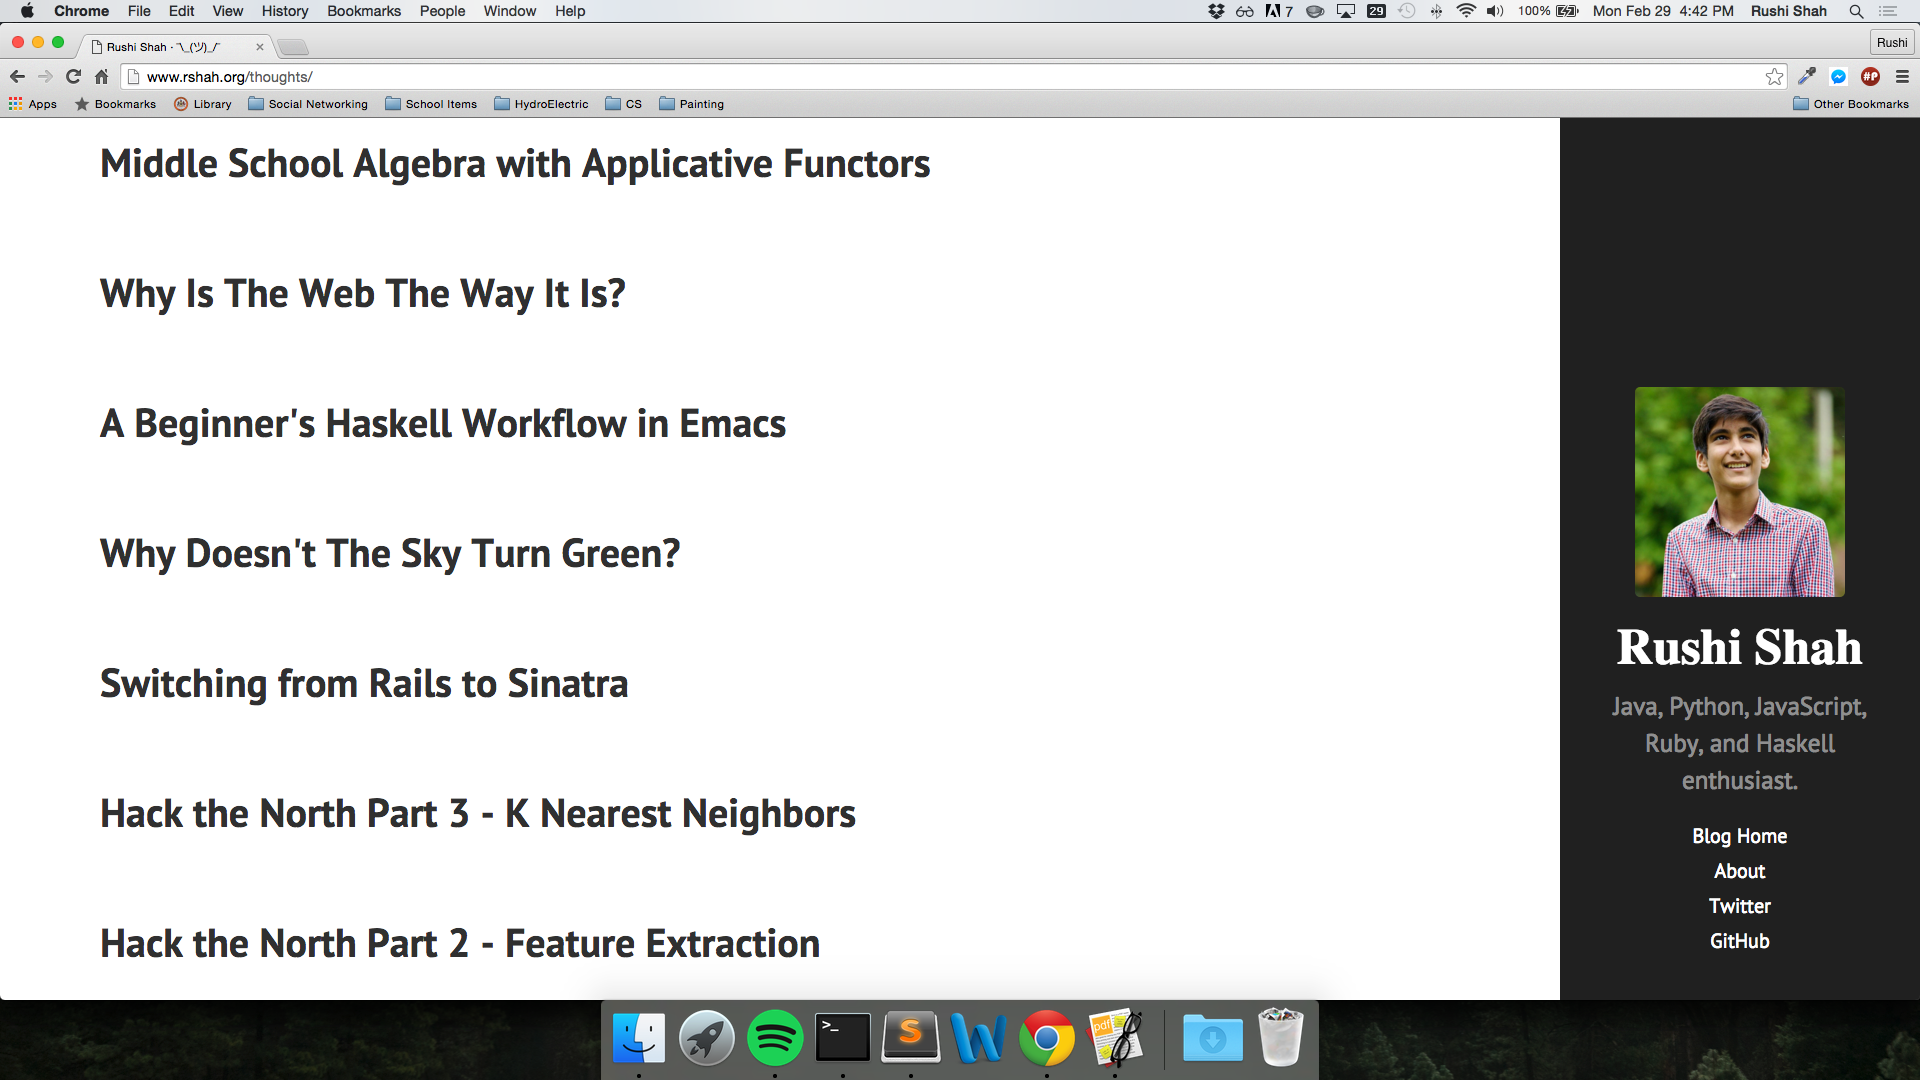
\includegraphics[width=.8\textwidth]{BlaTeX_screenshot}}

%-------------------------
 % Results, Discussion, Conclusion              
%-------------------------
\clearpage

\section{Results, Discussion, and Conclusion}

\subsection{Results}
This project resulted in a simple, configurable, and useful tool called BlaTeX that lets users write posts in a powerful typesetting language and compile their posts into a beautiful static-site. 

% It is designed to be simple and effective in all aspects from installation to usage.

\subsection{Discussion}
BlaTeX benefits mathemeticians, computer-scientists, and students of both disciplines who would like to maintain a technical blog about their work. It allows them to write their posts with the same advanced tools they use for their professional work. 

The project is also a milestone for the language used to write it. Often the popularity of computer science languages is based heavily on the amount of open-source projects implemented with that language. Haskell is often disparaged because it is rarely used for personal projects, however the Haskell community is trying to refute this claim. Thus, BlaTeX contributes to the growing population of popular projects implemented in Haskell and demonstrates that Haskell is a reasonable choice for future open-source projects. 

LaTeX is widely constrained to only being used in large-scale academic or professional projects, which is why it is such a mature piece of software. However BlaTeX broadens the scope of LaTeX itself by allowing people to utilize the strenght of LaTeX on a day-to-day basis. 

Future work can concentrate on the limitations outlined above, and specifically the fact that as of right now all posts are PDFs. Pandoc is a tool that converts between file formats (and is also written in Haskell). In order to address the potential limitation that BlaTeX doesn't produce HTML posts, further extensions could explore Pandoc conversions to HTML prior to static-site compilation. 

\subsection{Conclusion}
% The future of BlaTeX is in the open source community. Future maintenance will be based on issues reported on Github by actual users. The code will be distributed through Github as well, and users will be able to contribute to its development in the spirit of open-source.

BlaTeX was ultimately an experiment in niche fields. It caters to a (admittedly small) set of people who are either LaTeX enthusiasts, Haskell enthusiasts, or tech-savvy blogging enthusiasts. LaTeX is widely popular in certain fields (specifically math and computer-science), but virtually unknown past that. Haskell attracts fervent users who are passionate about and proud of the code they produce, but is not as popular as more main-stream languages like Java. It may seem like there are a lot of bloggers out there, but only a subset of them are tech-savvy enough to consider a software like this. These factors imply that BlaTeX would not be a very significant project: relevant to only a small population. But just because that population is small does not mean it does not mean it does not exist or can be ignored. Thus the significance of BlaTeX does not lie in its broad reach, but rather in its commitment to solve a very specific problem very well.  

% The specificity of the set of people who would like this project is precisely why it was successful. The significance of BlaTeX does not lie in its broad reach, but rather in its commitment to solve a very specific problem very well. 

%With that being said, the specificity of people who would find this project compelling is why it was successful. 

%The question was whether or not  Although the intersection of these two groups may seem rather insignificant, this project is useful to a group of people, which is significant. 

% % Presents the reader with the implication of the results.  
% Provide context so we can see what it all means.
% Provide specific, concise and thorough discussion of what you’ve learned.

%implications of results


%-------------------------
 % Citations and References              
%-------------------------

% Citation of Einstein paper~\cite{Einstein}. Citation of Freud book~\cite{Freud}.

% \bibliography{final}

\end{document}
